% =====================================================================
%  ARadhana — Project Documentation Template
%  Build:  pdflatex main && bibtex main && pdflatex main && pdflatex main
%  Structure mirrors docs/*.md so content can be ported section by section.
%  Every section file contains TODO markers — nothing is prefilled.
% =====================================================================
\documentclass[12pt,a4paper]{report}

% ---------- Layout ----------
\usepackage[a4paper,margin=1in]{geometry}
\usepackage{setspace}
\onehalfspacing
\usepackage{parskip}

% ---------- Fonts & language ----------
\usepackage[T1]{fontenc}
\usepackage[utf8]{inputenc}
\usepackage{lmodern}
\usepackage[english]{babel}

% ---------- Brand colors (match the app's Tailwind palette) ----------
\usepackage{xcolor}
\definecolor{orchidcrimson}{HTML}{DC143C}
\definecolor{orchidnavy}{HTML}{003893}
\definecolor{codegray}{HTML}{F5F4F0}
\definecolor{inkmuted}{HTML}{6B6558}

% ---------- Headings ----------
\usepackage{titlesec}
\titleformat{\chapter}[display]
  {\normalfont\huge\bfseries\color{orchidnavy}}
  {\color{inkmuted}\large Chapter \thechapter}{12pt}{\Huge}
\titlespacing*{\chapter}{0pt}{0pt}{28pt}
\titleformat*{\section}{\Large\bfseries\color{orchidnavy}}
\titleformat*{\subsection}{\large\bfseries}

% ---------- Header / footer ----------
\usepackage{fancyhdr}
\pagestyle{fancy}
\fancyhf{}
\fancyhead[L]{\small\color{inkmuted}ARadhana}
\fancyhead[R]{\small\color{inkmuted}\leftmark}
\fancyfoot[C]{\thepage}
\renewcommand{\headrulewidth}{0.3pt}

% ---------- Figures, tables, lists ----------
\usepackage{graphicx}
\graphicspath{{figures/}}
\usepackage{booktabs}
\usepackage{longtable}
\usepackage{enumitem}
\setlist{nosep}
\usepackage{caption}
\captionsetup{font=small,labelfont={bf,color=orchidnavy}}

% ---------- Code listings ----------
\usepackage{listings}
\lstdefinestyle{orchidcode}{
  backgroundcolor=\color{codegray},
  basicstyle=\ttfamily\small,
  keywordstyle=\color{orchidnavy}\bfseries,
  stringstyle=\color{orchidcrimson},
  commentstyle=\color{inkmuted}\itshape,
  numbers=left,
  numberstyle=\tiny\color{inkmuted},
  frame=single,
  rulecolor=\color{inkmuted!40},
  breaklines=true,
  showstringspaces=false,
  tabsize=2,
  captionpos=b,
}
\lstset{style=orchidcode}
% JSON has no built-in lexer — minimal definition for schema/API examples.
\lstdefinelanguage{json}{
  morestring=[b]",
  morekeywords={true,false,null},
  sensitive=true,
}

% ---------- Links (load last) ----------
\usepackage[hidelinks]{hyperref}
\hypersetup{
  pdftitle={ARadhana — Project Documentation},
  pdfauthor={TODO: team name},
  colorlinks=true,
  linkcolor=orchidnavy,
  urlcolor=orchidcrimson,
  citecolor=orchidnavy,
}

% ---------- Convenience macros ----------
\newcommand{\projectname}{ARadhana}
\newcommand{\todo}[1]{\textcolor{orchidcrimson}{\textbf{[TODO: #1]}}}
\newcommand{\code}[1]{\texttt{#1}}
% Usage: \apiroute{GET}{/api/visiting-places}
\newcommand{\apiroute}[2]{\code{\textcolor{orchidnavy}{\textbf{#1}} #2}}

% =====================================================================
\begin{document}

% ---------------- Title page ----------------
\begin{titlepage}
  \centering
  \vspace*{1.5cm}
  % \includegraphics[width=0.35\textwidth]{logo}\\[1cm]   % TODO: drop logo into figures/
  {\color{orchidcrimson}\rule{\textwidth}{2pt}}\\[1.2cm]
  {\Huge\bfseries\color{orchidnavy}\projectname}\\[0.4cm]
  {\Large AR-Guided Heritage \& Campus Exploration}\\[0.2cm]
  {\large\color{inkmuted}\todo{one-line tagline}}\\[1.2cm]
  {\color{orchidcrimson}\rule{\textwidth}{2pt}}\\[2cm]

  {\large\textbf{Project Documentation}}\\[2cm]

  \begin{tabular}{r l}
    \textbf{Team}       & \todo{team name}            \\[6pt]
    \textbf{Members}    & \todo{member 1}             \\
                        & \todo{member 2}             \\
                        & \todo{member 3}             \\[6pt]
    \textbf{Event}      & \todo{hackathon / course}   \\[6pt]
    \textbf{Institution}& \todo{institution}          \\[6pt]
    \textbf{Date}       & \today                      \\
  \end{tabular}

  \vfill
  {\small\color{inkmuted}\todo{footer note, e.g. supervisor / mentor}}
\end{titlepage}

% ---------------- Front matter ----------------
\pagenumbering{roman}

\chapter*{Abstract}
\addcontentsline{toc}{chapter}{Abstract}
\todo{150--250 word summary: what \projectname{} is, the problem it solves,
the approach (AR pathfinding + gamification), and the headline outcome.}

\vspace{1em}
\noindent\textbf{Keywords:} \todo{augmented reality, geofencing, gamification, \ldots}

\tableofcontents
\listoffigures
\listoftables
\clearpage

% ---------------- Main matter ----------------
\pagenumbering{arabic}

\chapter{Introduction}
\label{ch:introduction}
% Port from: docs/01_overview.md

\section{Background}
Nepal's cultural landscape is dense with sites worth exploring: the country
holds ten UNESCO World Heritage properties, four of them cultural sites within
the Kathmandu Valley alone, and it welcomed 1.147 million international
tourists in 2024. Yet the experience of actually visiting such a site --- or,
at a smaller scale, of a newcomer finding their way around a university
campus --- remains largely unassisted. Navigation applications reliably bring
a visitor to the entrance of a monument or an institution, but the guidance
ends at the gate. Inside, visitors depend on scarce physical tourism centres,
sparse signage, or the availability of a human guide.

At the same time, the technical preconditions for a software answer to this
gap have matured. Modern smartphones ship with GPS receivers, magnetometers,
and cameras as standard hardware, and web browsers now expose geolocation,
device orientation, and camera access directly to web pages, making
location-based Augmented Reality (AR) possible without installing a native
application. \projectname{} was built on this premise for Orchid HackX 2026
by Team Valhalla: a guided, gamified AR walk that begins where conventional
navigation stops.

\section{Project Overview}
\projectname{} is a mobile-first, gamified AR navigation platform for
educational campuses and heritage sites. A user opens the web application in
a smartphone browser, selects a pre-mapped route, and is guided in real time
by a live compass arrow together with a GPS distance readout to the next
waypoint. When the user physically arrives at a checkpoint, the system
detects their presence through geofencing and confirms the visit; only then
is the location-specific media for that checkpoint unlocked --- a video
testimonial, a historical image, or a narrative clip --- rendered anchored in
the real world through the device camera using an AR overlay.

Exploration is reinforced by a gamification layer. Users accumulate AR
Points through quiz answers, milestone completions, and side quests; earn
digital milestone badges for completing all milestone stops of a route;
answer five-question multiple-choice knowledge quizzes unlocked after
finishing a route; and compete on a community leaderboard. Points are
redeemable for tangible campus perks through a reward store, and optional
side quests reward detours that require a minimum five-minute on-site stay.

The platform is administered without code. An admin dashboard provides a
waypoint logger for defining route coordinates, waypoint types, and media; a
place management interface for creating, updating, and deleting visiting
places together with their cascaded route data; quiz management; user
management; and aggregate statistics. Because each place records a visitor
count as visits are confirmed, the system generates engagement analytics
organically, with no additional instrumentation.

\begin{figure}[ht]\centering
  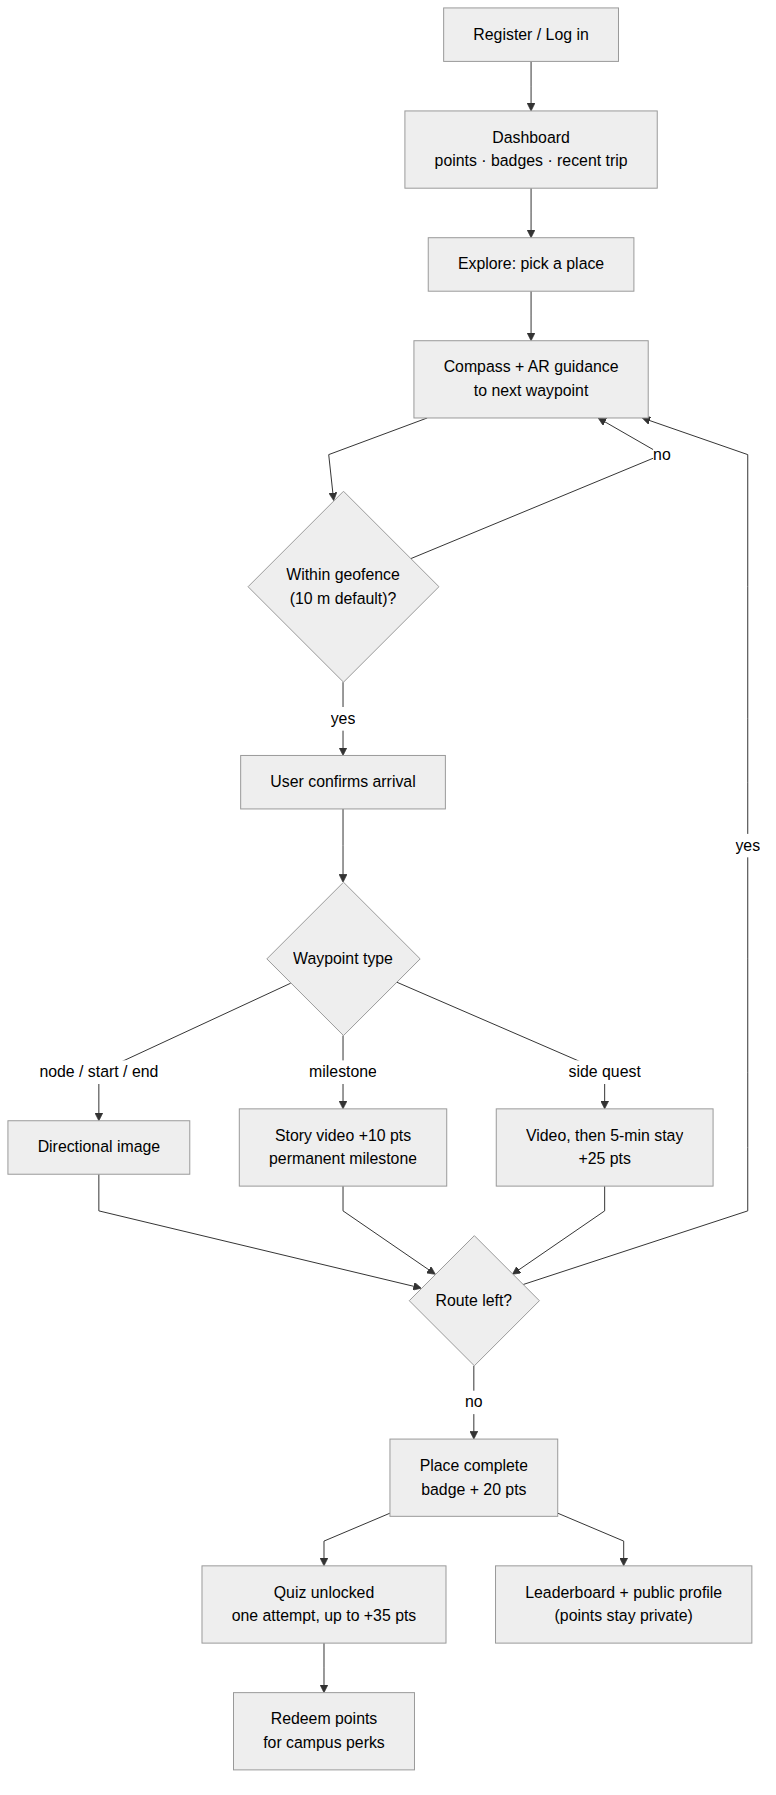
\includegraphics[height=0.8\textheight,width=\textwidth,keepaspectratio]{user-flow}
  \caption{End-to-end user journey: from registration to reward redemption.}\label{fig:userflow}
\end{figure}

\section{Scope}
This build delivers a complete vertical slice of the platform as a web
application, proven end-to-end on a single campus route at Orchid College in
Kathmandu. In scope are: route selection and real-time compass navigation;
geofence-verified checkpoint confirmation; AR media playback anchored in the
camera view; the full gamification loop (AR Points, milestones, side quests,
quizzes, badges, leaderboard, and reward redemption); and the complete admin
tooling required to configure routes, media, quizzes, and users.

Explicitly out of scope for this build are native mobile applications (the
product is browser-based only), offline operation (an active network
connection is required for the real-time proximity stream and media
delivery), and multi-language support (the interface is English-only). The
same infrastructure is designed to be pointed at other premises --- heritage
sites such as Pashupatinath or Boudhanath --- but only the Orchid College
route is demonstrated here.

\section{Report Organisation}
The remainder of this report is organised as follows.
\begin{itemize}
  \item Chapter~\ref{ch:problem-statement} states the problem the platform
        addresses and the motivation for solving it now.
  \item Chapter~\ref{ch:objectives} lists the general and specific
        objectives of the project.
  \item Chapter~\ref{ch:market-analysis} summarises the market context,
        competitive landscape, and target user segments.
  \item Chapter~\ref{ch:design-thinking} summarises the design process
        that shaped the product.
  \item Chapter~\ref{ch:system-architecture} describes the overall system
        architecture, from the browser client to the clustered backend.
  \item Chapter~\ref{ch:database-schemas} documents the database schema and
        the relationships between its collections.
  \item Chapter~\ref{ch:gamification} details the gamification
        engine: points, milestones, side quests, quizzes, badges, and
        rewards.
  \item Chapter~\ref{ch:ar-pathfinder} explains the AR pathfinder ---
        geofencing, the compass HUD, and the camera overlay.
  \item Chapter~\ref{ch:tech-stack} justifies the technology stack
        used across all layers.
  \item Chapter~\ref{ch:results} presents the results achieved during the
        hackathon build.
  \item Chapter~\ref{ch:future-work} discusses current
        limitations and future work.
  \item Chapter~\ref{ch:conclusion} concludes the report.
  \item Appendix~\ref{app:api} provides the API reference,
        Appendix~\ref{app:schemas} the field-level database schema
        reference, and Appendix~\ref{app:code} selected code listings.
\end{itemize}

\chapter{Problem Statement}
\label{ch:problem-statement}
% NOTE: intentionally blank — the earlier auto-generated problem statement
% was rejected. Write the real one here from scratch.

\todo{THE PROBLEM STATEMENT. Replace entirely --- do not reuse the
auto-generated draft. Suggested shape:
(1) the situation today and who is affected,
(2) the specific gap or pain point,
(3) why existing approaches fall short,
(4) the consequence of leaving it unsolved.}

\section{Motivation}
\todo{Why this problem is worth solving now, and why this team.}


\chapter{Objectives}
\label{ch:objectives}

\section{General Objective}
The general objective of this project is to build a self-guided,
geofence-verified AR exploration platform that makes heritage and campus
visits engaging, measurable, and scalable --- replacing the human-guided
tour with software that guides visitors in real time, verifies their
physical presence, and rewards exploration.

\section{Specific Objectives}
To realise the general objective, \projectname{} pursues the following
specific objectives:

\begin{itemize}
  \item \textbf{Verify physical presence via dynamic geofencing.} Detect and
        confirm a visitor's arrival at each waypoint using a geofence radius
        of 10~metres stored per place, so that visits, rewards, and
        analytics are grounded in verified presence rather than
        self-reporting.
  \item \textbf{Guide visitors in real time.} Provide continuous wayfinding
        to the next waypoint through a live compass heads-up display with a
        GPS distance readout, together with an AR camera overlay that
        anchors guidance in the visitor's view of the real world.
  \item \textbf{Unlock location-specific media on confirmed arrival.}
        Release each checkpoint's images and videos --- historical context,
        testimonials, and narrative clips --- only after the geofence has
        confirmed that the visitor is physically at the location.
  \item \textbf{Drive engagement through gamification.} Sustain exploration
        with AR Points, milestone completions, optional side quests,
        post-route knowledge quizzes, digital badges, a community
        leaderboard, and a store where points are redeemed for tangible
        perks.
  \item \textbf{Give administrators no-code control.} Allow site
        administrators to create and manage routes, waypoints, media,
        quizzes, and users entirely through a dashboard, with engagement
        analytics generated organically from per-place visitor counts.
  \item \textbf{Remain hardware-free and site-agnostic.} Run entirely in the
        smartphone browser with no physical installation at the site, so
        that the same platform can be configured for any campus, museum, or
        heritage property.
\end{itemize}

\chapter{Market Analysis}
\label{ch:market-analysis}
% Port from: docs/02_market_analysis.md

\section{Target Users}
\todo{Segments and their needs.}

\section{Existing Solutions}
\todo{Competitor / alternative overview table.}
% \begin{table}[h]\centering
%   \begin{tabular}{@{}lll@{}}\toprule
%   Solution & Strengths & Gaps \\ \midrule
%   \todo{...} & & \\ \bottomrule
%   \end{tabular}
%   \caption{Comparison of existing solutions}
% \end{table}

\section{Differentiation}
\todo{What \projectname{} does that the alternatives do not.}


\chapter{Design Thinking}
\label{ch:design-thinking}
% Port from: docs/03_design_thinking.md

\section{Empathise}
\todo{User research / assumptions.}

\section{Define}
\todo{Point-of-view statements.}

\section{Ideate}
\todo{Options considered.}

\section{Prototype \& Test}
\todo{What was prototyped, what feedback changed.}


\chapter{System Architecture}
\label{ch:system-architecture}
% Port from: docs/04_system_architecture.md

\section{High-Level Architecture}
\todo{Diagram + narrative: React client, Express File Cluster server,
MongoDB, WebSocket pathfinder channel.}
% \begin{figure}[h]\centering
%   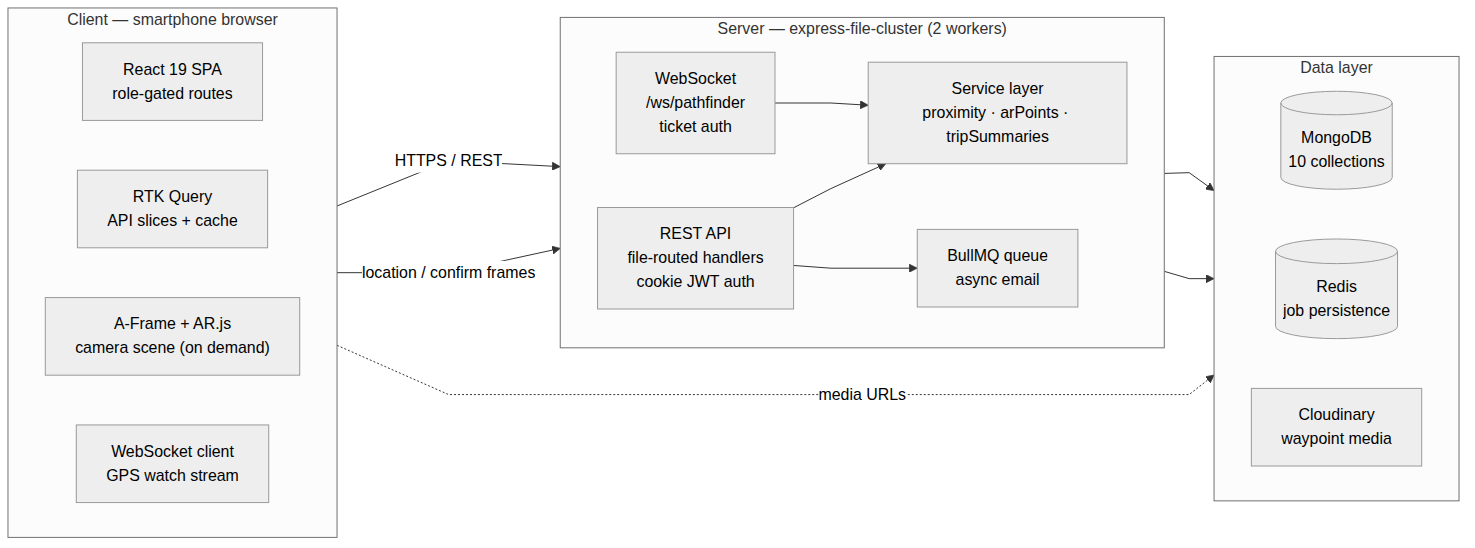
\includegraphics[width=\textwidth]{architecture}
%   \caption{System architecture}\label{fig:architecture}
% \end{figure}

\section{Client}
\todo{SPA structure, routing, role-based experience (user vs admin), RTK Query.}

\section{Server}
\todo{File-based routing, auth strategy, WebSocket proximity engine.}

\section{Real-Time Location Pipeline}
\todo{GPS watch $\rightarrow$ WS location frames $\rightarrow$ haversine
proximity $\rightarrow$ arrival confirmation $\rightarrow$ dynamic geofence
threshold served from the place record.}


\chapter{Database Design}
\label{ch:database-schemas}
% Port from: docs/05_database_schemas.md

\section{Entity Overview}
\todo{ER-style overview of User, VisitingPlace, VisitingRoutes, UserProgress,
Quiz, QuizAttempt, ArPoints.}

\section{Schema Reference}
\todo{One subsection per model; use lstlisting with language=json.}
% \begin{lstlisting}[language=json,caption={VisitingPlace schema}]
% { "name": "...", "visit_threshold_meters": 10, "visitor_count": 0 }
% \end{lstlisting}

\section{Denormalisation Decisions}
\todo{Why visitor\_count is a counter, why AR points are a ledger, badge
permanence via ledger + profile milestones.}


\chapter{Gamification Engine}
\label{ch:gamification}
% Port from: docs/09_gamification_engine.md

\section{AR Points}
\todo{Earning table: quiz 10/20/25/30/35, side quest 25, milestone 10,
place completion 20. Privacy: points are never public.}

\section{Quizzes}
\todo{One quiz per place, 5 questions, unlock-on-completion, single attempt,
answer review.}

\section{Badges \& Milestones}
\todo{Badge rules, permanence across revisits.}

\section{Leaderboard}
\todo{Metrics (milestones / places / side quests), why AR points are excluded.}

\section{Redemption}
\todo{Rewards catalog and the spend ledger.}


\chapter{AR Pathfinder}
\label{ch:ar-pathfinder}
% Port from: docs/10_ar_pathfinder.md

The pathfinder combines four real-time data streams --- GPS coordinates,
device compass heading, WebSocket proximity messages, and camera-based AR
rendering --- into one navigation experience. Code listings for the formulas
referenced here appear in Appendix~\ref{app:code}.

\section{Geofencing and Two-Phase Arrival}
All proximity checks run server-side using the haversine great-circle
formula, accurate to well under a metre at campus distances --- far finer
than the 3--5\,m accuracy of consumer GPS itself. A waypoint counts as
reached when the reported position falls within the place's geofence
radius. The radius --- the \code{visit\_threshold\_meters} field on the
place --- defaults to 10\,m rather than being hard-coded: dense
environments may need a
tighter fence to avoid false arrivals, open spaces a looser one to absorb
GPS drift, and administrators can tune it without a deployment.

Arrival is deliberately a two-phase process. Detection --- the server
reporting \code{arrived: true} --- only raises a confirmation prompt.
The checkpoint is marked visited only when the user explicitly confirms,
and the server re-validates the last reported position against the same
radius before accepting. A momentary GPS glitch therefore cannot complete a
checkpoint, and a confirmed visit is backed by two independent
within-radius checks.

\section{Compass Guidance}
The server includes a true-north bearing to the next waypoint in every
progress frame. The client subtracts the device's compass heading to obtain
the relative bearing that drives the HUD arrow. Two engineering details
make this usable. First, raw \code{DeviceOrientationEvent} readings jitter
by several degrees per frame, so headings pass through an exponential
moving average (weight 0.15 on the new reading) that removes jitter while
still responding to turns within about two seconds. Second, orientation
events arrive at up to 60\,Hz; routing them through React state would
re-render the component tree at that rate, so the arrow and distance text
are updated imperatively through refs, bypassing rendering entirely. iOS
additionally requires an explicit permission request for orientation data,
which is why navigation can only start from a button press (a user
gesture).

\section{AR Camera Layer}
The AR view uses A-Frame with AR.js location-based tracking, with the
camera feed rendered as a WebGL texture. The \code{<a-scene>} element is
injected directly under \code{<body>}, outside the React tree --- A-Frame
requires this to size its fullscreen canvas correctly --- and is fully torn
down (including stopping webcam tracks) when navigation ends. The vendor
scripts are served locally and loaded on demand only when AR mode starts,
which pins versions (A-Frame 1.6.0, AR.js 3.4.7), avoids ad-blocker
interference, and keeps the initial page load small.

Milestone and side-quest videos play on a plane anchored in world space.
Anchoring by GPS coordinates would make the plane jump with satellite
drift, so instead the plane spawns four metres in front of the camera, its
rotation frozen at spawn (looking around pans off it, as with a real
object), while its position is re-glued to the camera's translation every
animation frame. The result reads as ``placed in the world'' yet is immune
to GPS jitter.

\section{Waypoint Types}
\begin{table}[h]
  \centering\small
  \begin{tabular}{@{}lp{0.68\textwidth}@{}}
    \toprule
    \textbf{Type} & \textbf{Behaviour on arrival} \\
    \midrule
    \code{start} & Confirmation prompt; opening image shown \\
    \code{node} & Turn point; directional image shown on confirmation \\
    \code{milestone} & Video plays; confirmation awards points and logs the milestone \\
    \code{side\_quest} & Video plays; accept starts the 5-minute dwell timer, skip continues \\
    \code{end} & Final checkpoint; completion image and trip-complete state \\
    \bottomrule
  \end{tabular}
  \caption{Waypoint type semantics.}
  \label{tab:waypoints}
\end{table}

\section{Graceful Degradation and Demo Mode}
The design principle is that the compass arrow is always the fallback.
Without HTTPS (camera APIs require a secure context) or if the AR scripts
fail to load, navigation continues with the compass HUD and a visible
notice; if video autoplay is blocked, a tap-to-play overlay appears; if the
compass reports non-absolute headings, a calibration banner is shown.
A separate demo mode bypasses GPS entirely: it replays the real route from
hardcoded waypoints with a ``simulate arrival'' control, exercising the
complete flow --- media, confirmations, rewards UI --- indoors, which is
essential for stage demonstrations and QA.

\section{The Seeded Route}
The production route walks Orchid College over approximately 400\,m
(five to seven minutes): a start point, three turn nodes, two milestones
with video stories (the parking area and Orchid International College), one
side quest (Bishwajit Medical Hall), and an end point, with a 10\,m
geofence per waypoint and the college badge on completion.

\chapter{Technology Stack}
\label{ch:tech-stack}
% Port from: docs/08_packages.md

\section{Frontend}
\todo{React 19, Redux Toolkit Query, Tailwind CSS 4, lucide-react,
cartoon-avatar, A-Frame/AR.js.}

\section{Backend}
\todo{Express File Cluster, MongoDB/mongoose, ws, jose, bcrypt.}

\section{Tooling}
\todo{Vite, TypeScript, ESLint, tsx.}


\chapter{Results}
\label{ch:results}

\section{Delivered Features}
The hackathon build delivers a complete vertical slice, working end to end:

\begin{itemize}
  \item \textbf{Exploration.} Route selection, live compass HUD with
        distance readout, AR camera overlay with world-anchored story
        videos, geofence-verified two-phase checkpoint confirmation, media
        unlocks per waypoint type, side-quest dwell timer, revisit with
        progress reset, and a GPS-free demo mode.
  \item \textbf{Gamification.} Private AR~Points ledger with idempotent
        awards, permanent milestone log and badges, per-place quizzes with
        completion lock, single attempt, and answer review, and a rewards
        catalog with confirm-before-spend redemption.
  \item \textbf{Community.} Public profiles, a people directory with
        debounced search, and a leaderboard ranked by milestones, places,
        or side quests with AR~Points kept private.
  \item \textbf{Administration.} A role-separated admin experience:
        statistics dashboard with 30-day signup and milestone trends, user
        management (verify, suspend, reactivate, promote, delete), the
        waypoint logger for route authoring, and per-place quiz and
        geofence-radius configuration.
\end{itemize}

\section{Field Test}
The complete loop was validated on the seeded Orchid College route
(eight waypoints, $\sim$400\,m) and a second short route at the hackathon
venue. Real users registered, walked the routes, and confirmed checkpoints:
arrival prompts fired inside the 10\,m geofence, confirmations persisted
across sessions, milestone videos played anchored in the camera view, the
side-quest timer enforced the five-minute stay, badges and completion
points were awarded exactly once per user, quizzes unlocked only after
completion, and redeemed rewards appeared as negative ledger entries. The
place visitor counters advanced once per unique completer, and the admin
dashboard reflected the activity without any manual instrumentation.

\section{Screenshots}
Screenshots of the main surfaces (explore, AR navigation, quiz, redemption,
leaderboard, and admin dashboard) are to be captured from the deployed
build and inserted here.

% \begin{figure}[h]\centering
%   \includegraphics[width=0.45\textwidth]{screen-explore}\hfill
%   \includegraphics[width=0.45\textwidth]{screen-ar}
%   \caption{Explore page and AR navigation.}\label{fig:screens-1}
% \end{figure}
% \begin{figure}[h]\centering
%   \includegraphics[width=0.45\textwidth]{screen-quiz}\hfill
%   \includegraphics[width=0.45\textwidth]{screen-redeem}
%   \caption{Quiz review and rewards redemption.}\label{fig:screens-2}
% \end{figure}
% \begin{figure}[h]\centering
%   \includegraphics[width=0.45\textwidth]{screen-leaderboard}\hfill
%   \includegraphics[width=0.45\textwidth]{screen-admin}
%   \caption{Community leaderboard and admin dashboard.}\label{fig:screens-3}
% \end{figure}

\chapter{Limitations \& Future Work}
\label{ch:future-work}

\section{Known Limitations}
\todo{GPS accuracy vs 10 m geofence, HTTPS requirement for camera,
avatar CDN dependency, \ldots}

\section{Future Work}
\todo{Roadmap items.}


\chapter{Conclusion}
\label{ch:conclusion}

\todo{Close the loop: restate the problem, what was built, what it proves.}



% ---------------- References ----------------
\nocite{*} % template: list all .bib entries even before anything is cited
\bibliographystyle{ieeetr}
\bibliography{references}
\addcontentsline{toc}{chapter}{References}

% ---------------- Appendices ----------------
\appendix
\chapter{API Reference}
\label{app:api}
% Port from: docs/06_api_reference.md

\todo{Endpoint tables grouped by area. Example row format:}

% \begin{longtable}{@{}lll@{}}\toprule
% Endpoint & Auth & Description \\ \midrule
% \apiroute{GET}{/api/visiting-places} & user, admin & List places \\
% \bottomrule
% \caption{Visiting places endpoints}
% \end{longtable}


\chapter{Folder Structure}
\label{app:folders}
% Port from: docs/07_folder_architecture.md

\todo{Annotated tree of client/ and server/.}
% \begin{lstlisting}
% server/src/
%   api/          file-based routes
%   lib/          proximity, points, trip summaries
%   model/        mongoose-backed models
% \end{lstlisting}



\end{document}
